\documentclass[11pt]{article}
\usepackage[utf8]{inputenc}
\usepackage[T1]{fontenc}
\usepackage{amsmath}
\usepackage{amssymb} % Needed for \eth
\usepackage{graphicx}
\usepackage{geometry}
\usepackage{tikz}
\usepackage{pgfplots} % For plots
\usepackage{ulem}     % For underline, using normalem to avoid messing with \emph
\usepackage{tcolorbox} % For boxing equations
\usepackage{braket}    % For QM state notation if needed

\geometry{a4paper, margin=1in}
\usetikzlibrary{positioning, arrows.meta, shapes.geometric} % For TikZ diagrams
\pgfplotsset{compat=1.18} % Use a recent PGFPlots version

% Custom commands (optional)
\newcommand{\avg}[1]{\overline{#1}}
\newcommand{\prob}[1]{P(#1)}
\newcommand{\ProbDens}[1]{\mathcal{P}(#1)} % Using script P for density
\newcommand{\vect}[1]{\vec{#1}}
\newcommand{\dd}[1]{\mathrm{d}#1} % Differential d
\newcommand{\pderiv}[2]{\frac{\partial #1}{\partial #2}}
\newcommand{\deriv}[2]{\frac{\mathrm{d} #1}{\mathrm{d} #2}}
\newcommand{\muState}{\mu\text{-state}} % Microstate
\newcommand{\OmegaE}{\Omega(E)}
\newcommand{\omegaE}{\omega(E)}
\newcommand{\PhiE}{\Phi(E)}
\newcommand{\deltaE}{\delta E}
\newcommand{\ethbar}{\text{\it{đ}}} % \eth symbol for inexact differential
\newcommand{\kb}{k_B} % Boltzmann constant
\newcommand{\gasR}{R} % Ideal gas constant
\newcommand{\partfn}{Z} % Partition function symbol

% Define a tcolorbox style for boxed equations
\tcbuselibrary{skins}
\newtcolorbox{eqbox}[1][]{
  enhanced,
  colback=yellow!10!white,
  colframe=blue!75!black,
  boxrule=1pt,
  arc=3mm,
  #1
}

\title{Physics 415 - Lecture 19: Canonical Ensemble Properties}
\date{March 5, 2025}
\author{} % Author not specified

\begin{document}

\maketitle
\thispagestyle{empty}

\section*{Summary: Ensembles}

\begin{description}
    \item[Microcanonical Ensemble (MCE):]
    \begin{itemize}
        \item Describes closed, isolated system.
        \item $E=$ fixed (or in range $(E, E+\deltaE)$), $N, V$ fixed.
        \item $P_r = \begin{cases} 1/\Omega(E) & \text{if } E < E_r < E+\deltaE \\ 0 & \text{else} \end{cases}$. (Equal probability for accessible states).
        \item $S = \ln \Omega$.
    \end{itemize}

    \item[Canonical Ensemble (CE):]
    \begin{itemize}
        \item Describes system in thermal contact with heat reservoir at $T$.
        \item $T=$ fixed, $N, V$ fixed. Energy $E_r$ fluctuates.
        \item $P_r = \frac{e^{-E_r/T}}{\partfn} = \frac{e^{-\beta E_r}}{\partfn}$. (Canonical/Gibbs distribution).
        \item Partition function: $\partfn = \sum_r e^{-E_r/T} = \sum_r e^{-\beta E_r}$. ($\beta \equiv 1/T$).
    \end{itemize}
\end{description}

\section*{Example: Spin-1/2 in Magnetic Field (Canonical Ensemble)}

Consider a single spin-1/2 particle (magnetic moment $\mu$) in contact with a heat reservoir at temperature $T$, placed in an external magnetic field $H$ (along z-axis).
Let $m = \pm 1/2$ be the spin projection along $H$.
There are two microstates ($r=\pm$):
\[ E_\pm = \mp \mu H \]
The partition function $Z$ is:
\[ \partfn = \sum_{r=\pm} e^{-\beta E_r} = e^{-\beta E_+} + e^{-\beta E_-} = e^{\beta \mu H} + e^{-\beta \mu H} = 2 \cosh(\beta \mu H) \]
The probabilities of the two states are:
\[ P_\pm = \frac{e^{-\beta E_\pm}}{\partfn} = \frac{e^{\pm \beta \mu H}}{2 \cosh(\beta \mu H)} \]
Note the probabilities depend on the dimensionless parameter $x = \beta \mu H = \mu H / T$, the ratio of magnetic energy to thermal energy.
\begin{itemize}
    \item High $T$ ($x \ll 1$): $P_+ \approx P_- \approx 1/2$. Both states equally likely.
    \item Low $T$ ($x \gg 1$): $P_+ \approx e^x / (e^x+e^{-x}) \to 1$. $P_- \approx e^{-x} / (e^x+e^{-x}) \to 0$. Ground state ($m=+1/2$, spin aligned with field) dominates.
\end{itemize}

Average magnetic moment $\avg{\mu_z}$:
The moment in state $r$ is $\mu_r = m \times (2\mu) = \pm \mu$. % Factor of 2 is conventional for spin-1/2 moment
\[ \avg{\mu_z} = \sum_{r=\pm} P_r \mu_r = P_+ (+\mu) + P_- (-\mu) = \mu (P_+ - P_-) \]
\[ \avg{\mu_z} = \mu \frac{e^{\beta \mu H} - e^{-\beta \mu H}}{2 \cosh(\beta \mu H)} = \mu \frac{2 \sinh(\beta \mu H)}{2 \cosh(\beta \mu H)} = \mu \tanh(\beta \mu H) \]
\[ \implies \avg{\mu_z} = \mu \tanh\left(\frac{\mu H}{T}\right) \]

If the system has $n$ such non-interacting spins per unit volume, the magnetization density is $M = n \avg{\mu_z}$:
\[ M = n \mu \tanh\left(\frac{\mu H}{T}\right) \]

\begin{center}
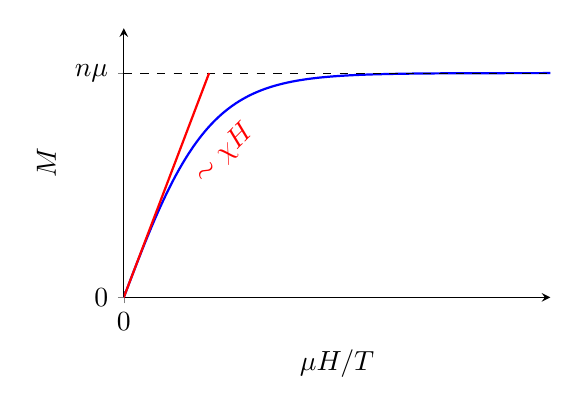
\begin{tikzpicture}
\begin{axis}[
    xlabel={$\mu H / T$}, ylabel={$M$},
    xmin=0, xmax=5, ymin=0, ymax=1.2,
    xtick={0}, ytick={0, 1}, yticklabels={$0$, $n\mu$},
    axis lines=left, width=7cm, height=5cm
]
\addplot [domain=0:5, samples=100, smooth, thick, blue] {tanh(x)};
\draw [dashed] (axis cs:0, 1) -- (axis cs:5, 1); % Saturation value
\draw [red, thick, domain=0:1] plot (\x, {\x}); % Linear approx at low field
\node at (axis cs:0.8, 0.5) [anchor=west, rotate=45, red] {$\sim \chi H$};
\end{axis}
\end{tikzpicture}
\end{center}

At low fields / high temperatures ($\mu H \ll T$, or $x \ll 1$), we can use $\tanh x \approx x$:
\[ M \approx n \mu \left( \frac{\mu H}{T} \right) = \frac{n \mu^2}{T} H = \chi H \]
where $\chi = \frac{n \mu^2}{T}$ is the magnetic susceptibility.
This result $\chi \propto 1/T$ is Curie's Law for paramagnetic materials.

\section*{Properties Derived from Partition Function Z}

Knowledge of $Z$ allows us to obtain statistical averages.

\subsection*{Average Energy $\avg{E}$}
\[ \avg{E} = \sum_r P_r E_r = \frac{1}{\partfn} \sum_r E_r e^{-\beta E_r} \]
Note that $\frac{\partial}{\partial \beta} e^{-\beta E_r} = -E_r e^{-\beta E_r}$.
\[ \implies \sum_r E_r e^{-\beta E_r} = -\frac{\partial}{\partial \beta} \sum_r e^{-\beta E_r} = -\pderiv{\partfn}{\beta} \]
\[ \avg{E} = \frac{1}{\partfn} \left( -\pderiv{\partfn}{\beta} \right) = -\frac{1}{\partfn} \pderiv{\partfn}{\beta} \]
This can be written compactly as:
\begin{eqbox}
\[ \avg{E} = -\pderiv{}{\beta} (\ln \partfn) \]
\end{eqbox}

\textbf{Check for spin-1/2 example:}
$\ln Z = \ln(2 \cosh(\beta \mu H))$.
$\avg{E} = \sum P_r E_r = P_+(-\mu H) + P_-(+\mu H) = -\mu H (P_+ - P_-) = -\mu H \tanh(\beta \mu H)$.
Also, $-\partial(\ln Z)/\partial \beta = -\frac{1}{Z} \frac{\partial Z}{\partial \beta} = -\frac{1}{2\cosh(\beta\mu H)} [2 \sinh(\beta\mu H) \times (\mu H)] = -\mu H \tanh(\beta \mu H)$. Matches. $\checkmark$

We can also relate average moment to $Z$:
$\avg{\mu_z} = \frac{1}{Z} \sum \mu_r e^{-\beta E_r} = \frac{1}{Z} \sum \mu_r e^{\beta \mu_r H}$.
$\frac{\partial Z}{\partial H} = \frac{\partial}{\partial H} \sum e^{\beta \mu_r H} = \sum \beta \mu_r e^{\beta \mu_r H}$.
So $\sum \mu_r e^{\beta \mu_r H} = \frac{1}{\beta} \frac{\partial Z}{\partial H} = T \frac{\partial Z}{\partial H}$.
$\avg{\mu_z} = \frac{1}{Z} (T \frac{\partial Z}{\partial H}) = T \frac{\partial (\ln Z)}{\partial H}$.

\subsection*{Energy Fluctuations}
The variance (dispersion) of energy is $\overline{\Delta E^2} = \avg{E^2} - (\avg{E})^2$.
\[ \avg{E^2} = \sum_r P_r E_r^2 = \frac{1}{\partfn} \sum_r E_r^2 e^{-\beta E_r} \]
Note $\frac{\partial^2}{\partial \beta^2} e^{-\beta E_r} = (-E_r)^2 e^{-\beta E_r} = E_r^2 e^{-\beta E_r}$.
\[ \implies \avg{E^2} = \frac{1}{\partfn} \pderiv[2]{\partfn}{\beta} \]
Now calculate $\overline{\Delta E^2}$:
\[ \overline{\Delta E^2} = \frac{1}{\partfn} \pderiv[2]{\partfn}{\beta} - \left( -\frac{1}{\partfn} \pderiv{\partfn}{\beta} \right)^2 = \frac{1}{\partfn} \pderiv[2]{\partfn}{\beta} - \frac{1}{\partfn^2} \left( \pderiv{\partfn}{\beta} \right)^2 \]
Consider $\pderiv{}{\beta} \avg{E} = \pderiv{}{\beta} \left( -\frac{1}{\partfn} \pderiv{\partfn}{\beta} \right) = \frac{1}{\partfn^2} \left( \pderiv{\partfn}{\beta} \right)^2 - \frac{1}{\partfn} \pderiv[2]{\partfn}{\beta} = - \overline{\Delta E^2}$.
So, $\overline{\Delta E^2} = -\pderiv{\avg{E}}{\beta}$.
This can also be written as:
\[ \overline{\Delta E^2} = \pderiv[2]{}{\beta} (\ln \partfn) \]

We can relate this to the heat capacity $C_V$. (Implicitly, V is fixed in the definition of $E_r$).
\[ \pderiv{\avg{E}}{\beta} = \pderiv{\avg{E}}{T} \pderiv{T}{\beta} \]
Since $T = 1/\beta$, $\partial T / \partial \beta = -1/\beta^2 = -T^2$.
Also, $(\partial \avg{E} / \partial T)_V = C_V$.
\[ \pderiv{\avg{E}}{\beta} = C_V (-T^2) = -T^2 C_V \]
So, $\overline{\Delta E^2} = -\pderiv{\avg{E}}{\beta} = T^2 C_V$.
\begin{eqbox}
\[ \overline{\Delta E^2} = T^2 C_V \]
\end{eqbox}
The energy fluctuations in the canonical ensemble are related to the heat capacity (the ability of the system to absorb heat).

\textbf{Sharpness of $P(E)$:}
We can now quantify the width $\Delta^* E$ of the energy distribution $P(E) \propto \Omega(E)e^{-\beta E}$. The width is related to the root-mean-square fluctuation:
\[ \Delta^* E = \sqrt{\overline{\Delta E^2}} = \sqrt{T^2 C_V} = T \sqrt{C_V} \]
The relative width is:
\[ \frac{\Delta^* E}{\avg{E}} = \frac{T \sqrt{C_V}}{\avg{E}} \]
Since $\avg{E}$ and $C_V$ are extensive quantities (proportional to $N$, the number of particles or DOF), while $T$ is intensive: $\avg{E} \propto N$, $C_V \propto N$.
\[ \frac{\Delta^* E}{\avg{E}} \propto \frac{\sqrt{N}}{N} = \frac{1}{\sqrt{N}} \]
The relative width of the energy distribution is vanishingly small for macroscopic systems ($N \sim 10^{23}$).

\textbf{Example:} Monatomic ideal gas.
$E = \frac{3}{2} N T$, $C_V = (\partial E/\partial T)_V = \frac{3}{2} N$. (Using $T$ in energy units, $k_B=1$).
\[ \frac{\Delta^* E}{\avg{E}} = \frac{T \sqrt{3N/2}}{(3/2)NT} = \frac{\sqrt{3N/2}}{(3/2)N} = \sqrt{\frac{3N/2}{9N^2/4}} = \sqrt{\frac{2}{3N}} \]
This scales as $1/\sqrt{N}$.

\section*{Thermodynamics in the Canonical Ensemble}

To analyze thermodynamic relations, we adopt a generalization of the entropy $S=\ln \Omega$ from the MCE. We define the \textbf{Gibbs entropy}:
\[ S = -\sum_r P_r \ln P_r \]
Here $P_r$ can be the probability distribution over microstates $r$ in any ensemble.

First, check that this recovers the familiar entropy in the MCE.
In MCE, $P_r = 1/\Omega(E)$ for $\Omega$ accessible states, and $P_r=0$ otherwise.
\[ S_{MCE} = -\sum_{r=1}^{\Omega} \frac{1}{\Omega} \ln\left(\frac{1}{\Omega}\right) = -\sum_{r=1}^{\Omega} \frac{1}{\Omega} (-\ln \Omega) = \frac{\ln \Omega}{\Omega} \sum_{r=1}^{\Omega} (1) = \frac{\ln \Omega}{\Omega} \times \Omega = \ln \Omega \]
It recovers the previous definition. $\checkmark$

Now apply to the Canonical Ensemble (CE). $P_r = e^{-\beta E_r} / Z$.
$\ln P_r = \ln(e^{-\beta E_r}) - \ln Z = -\beta E_r - \ln Z$.
\[ S_{CE} = -\sum_r P_r \ln P_r = -\sum_r P_r (-\beta E_r - \ln Z) \]
\[ S_{CE} = \beta \sum_r P_r E_r + (\ln Z) \sum_r P_r \]
Using $\avg{E} = \sum P_r E_r$ and $\sum P_r = 1$:
\[ S = \beta \avg{E} + \ln Z \]
Since $\beta = 1/T$:
\[ S = \frac{\avg{E}}{T} + \ln Z \]
Rearranging: $\avg{E} - TS = -T \ln Z$.
The left side is exactly the definition of the Helmholtz Free Energy $F = E - TS$ (using the average energy $\avg{E}$ in the CE).
\begin{eqbox}
\[ F = -T \ln Z \]
\end{eqbox}
This is a fundamental result connecting statistical mechanics (the partition function $Z$, containing microscopic information $E_r$) to thermodynamics (the macroscopic potential $F$).
Compare with $S = \ln \Omega$ in the MCE. $F$ plays a role in the CE analogous to $S$ in the MCE.

\end{document}